\documentclass[10pt,a4paper]{article}
% for margining standards
\usepackage[left=3cm,right=3cm,top=3cm,bottom=3cm]{geometry}
% for counting references as a section
\usepackage[numbib,notlof,notlot,nottoc]{tocbibind}
% useful packages
\usepackage{
                graphicx, setspace, fontspec, caption,
                subcaption, float, polyglossia, rotating,
                lscape, pdflscape, indentfirst, tocloft,
                multirow, mathtools, currfile
            }
\usepackage[justification=centering]{caption}
% paragraph related package
\usepackage[parfill]{parskip}
% use bzar font(THIS MUST BE LOADED BEFORE XePerian PACKAGE)
\setmainfont{BZar.ttf}
% the dear XePersian package
\usepackage{xepersian}
%
% General settings goes here.
%
% lines space
\renewcommand{\baselinestretch}{1.5}
% paragraph first line indention
\setlength{\parindent}{1cm}
% paragraph spacing
\setlength{\parskip}{1em}
% set graphics' path
\graphicspath{ {images/} }
% make table of content dotted
\renewcommand{\cftsecleader}{\cftdotfill{\cftdotsep}}
% define a new command as {half-space} in english
\newcommand{\halfspace}{\hspace{0pt}}
% define a new command as {half-space} in persian
\newcommand{\نیمفاصله}{\halfspace}
% define a shortcut for half-space in general
\renewcommand{\ }{\halfspace}
% define a new command for ease of use for rendering reference
\newcommand{\renderref}[1] { \begingroup \let\clearpage\relax \include{#1} \endgroup }
\newcommand{\مق}{\lr}
\newcommand{\قم}{یادگیری تقویتی }
\newcommand{\ز}{\footnote{\lr{}}}
%
% DOCUMENT BEGIN
%
\begin{document}
\title{
    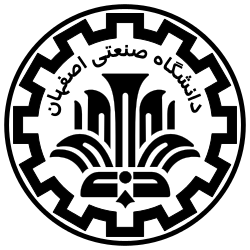
\includegraphics[width=.2\textwidth]{iut}\\
    گزارش سمینار درس یادگیری ماشین\\
یادگیری تقویتی در محیط\ های پیوسته در چند کاربرد
}
\author{داریوش حسن\ پور آده}
\date{۹۳۰۸۱۶۴}
\maketitle
\قسمت{مقدمه}
در حالت کلی یادگیری تقویتی شامل ۳ قسمت می\ باشد: عامل، محیط و اعمال که عامل همان موجودیتی می\ باشد که تصمیم می\ گیرد در محیط چه عملی را از میان اعمال تعریف شده برای خود به اجرا در آورد. محیط نیز در بازخورد به اعمالی که عامل انجام می\ دهد واکنش می\ دهد که این واکنش به عنوان امتیاز در یادگیری تقویتی تعریف شده است. هدف کلی از این زمینه تحقیق در مورد روش\ هایی که بتواند عامل با توجه به پاداش\ های دریافتی سیاست بهینه\ ی مرتبط با محیط را یاد بگیرد. در اکثر مسائل دنیای واقعی دنیا ربات(عامل) در محیطی پیوسته با موقعیت\ ها و اعمال پیوسته فعالیت می\ کند برای همین روش\ های متعارف ارائه شده برای یادگیری تقویتی در این\ گونه محیط\ های پیوسته قابل پیاده\ سازی نیست؛ بنابراین در این گزارش به معرفی تعدادی از کاربردهای پیوسته\ ی یادگیری تقویتی و روش\ هایی که برای این کاربردها ارائه شده است که بتوان یادگیری تقویتی را در مسائل پیوسته استفاده کرد. در این گزارش بنابه اینکه در دستور کار سمینار آورده شده است که باید دو مقاله بررسی شود به معرفی دو روشی که در مقالات آورده شده است پرداخته و به تحلیل نتایج حاصل از این روش\ ها می\ پردازیم و در نهایت از بحث\ های آورده شده نتیجه\ گیری\ ای خواهد شد.\بند
\noindent\textbf{کلیدواژه\ ها:}
یادگیری تقویتی، محیط\ ها و اعمال پیوسته
\newpage
\tableofcontents
\listoffigures
\listoftables
\newpage
\قسمت{تعریف مساله}
همان\ طور که قبلا گفته شد کلیه\ ی الگوریتم\ های یادگیری تقویتی بر مبنای «موقعیت، عمل، پاداش» عمل می\ کنند بدین\ گونه که عامل در موقعیتی خاص تصمیم می\ گیرد که یکی از اعمال ممکن و تعریف شده برایش را اجرا کند می\ کند و براساس آن عمل یک بازخوردی از محیط دریافت می\ کند که معمولا این بازخورد به صورت پاداش در نظر گرفته می\ شود\زیرنویس{دقت شود که در دنیای واقعی، \زیرخط{محیط} نمی\ توانند پاداشی به عامل بدهد، مگر اینکه توسط آموزگار این پاداش ارائه شود(که در حالت کلی آموزگار و محیط دو مفهوم مجزا هستند).}. در تعریف محیط\ های پیوسته در \قم پیوسته، به محیط\ هایی گفته می\ شود که یکی از یا هردوی «موقعیت» و «اعمال» شامل مقادیر پیوسته باشند. به عوان مثال می\ توان یادگیری ربات چهارپره را در نظر گرفت که موقعیت مکانی و زاویه\ ای و سرعت\ های خطی و زاویه\ ای ربات شامل مقادیر پیوسته می\ باشد که که موقعیت ربات در هرلحظه تعیین می\ کنند و اعمالی که چهارپره می\ تواند انجام دهد شامل سرعت\ هایی است که می\ تواند در هر لحظه به پره\ های خود بدهد می\ باشد. همان\ طور که می\ بینیم در این مثال هردوی موقعیت و اعمال شامل مقادیر پیوسته می\ باشند،‌ به همین خاطر روش\ های مرسوم یادگیری تقویتی نمی\ توانند برای این مورد استفاده شود زیرا که به\ تعداد نامتناهی موقعیت و اعمال داریم و روش\ های عادی نمی\ تواند به ازای تعداد نامتنهایی موقعیت و اعمال سیاست بهینه را یادگیری بگیرد.
\قسمت{انگیزه}
در مورد مشکلات کاربردهای دنیای واقعی با یادگیری تقویتی می\ توان گفت که، یک اینکه برای یادگیری یک سیاست بهینه حداقل چند هزار دور ربات باید اجرا شود که در دنیای واقعی معمولا این مساله ممکن نیست زیرا که هر اجرای ربات نیازمند زمان است، و این زمان هرچند اندک(حتی در حتی ۱-۲ ثانیه) به ازای چندهزار بار اجرا عملا قابل اجرا نیست، دوم اینکه چون در ابتدای کار یادگیری اکتشاف بیشتر رخ می\ دهد بنابراین ممکن است ربات در طی این اکتشاف\ ها با اجرای اعمال خطرناک به خود یا دیگران صدمه بزند و همچنین میزان زمان کالیبره کردن سنسورها بعد از اجرای هر دوره\ز{Epoch} زمان\ گیر و دردسرساز می\ باشد، به خاطر این دلایل از \قم در ربات\ های واقعی معمولا استفاده نمی\ شوند.\بند
علاوه\ بر مشکلات که ذکر شد که چرا یادگیری تقویتی در حالت کلی در رباتیک کاربرد ندارند مشکلاتی دیگر نیز وجود دارند که چرا \قم برای محیط\ های پیوسته کابرد ندارد می\ توان به ۳ مورد کلی «زمان، حافظه و عدم تضمین هم\ گرایی» اشاره کرد، علت دو مورد اول بدیهی است، زیرا که زمانی که با محیط\ های پیوسته درگیر می\ شویم یکی یا هردوی «موقعیت یا اعمال» به تعداد نامتناهی خواهیم داشت که بعد از اجرا الگوریتم خیلی طول نمی\ کشد که حافظه پر می\ شود، حتی اگر حافظه هم پر نشود چون تعداد نامتناهی است زمان یادگیری سیاست بهینه نیز نامتناهی می\ شود. علت مورد سوم را نیز می\ توان به صورت نشان داده، در اثبات هم\ گرایی یادگیری تقویتی آمده است که اگر بینهایت بار هر یکی از موقعیت-عمل\ ها را مشاهده کنیم در نهایت می\ توانیم به سیاست بهینه برسیم، ولی زمانی که تعداد موقعیت-عمل نامتناهی باشد، دیگر نمی\ توان یک تعداد نامتناهی را به تعداد دفعات نامتناهی مشاهده کنیم که بتوانیم سیاست بهینه را یاد بگیرد.\بند
در مورد راه\ حل\ های احتمالی برای \قم در محیط\ های پیوسته می\ توان به موارد «گسسته\ سازی»، «مدل\ سازی و یادگیری مدل»، «کاهش ابعاد»، «یادگیری توزیع\ شده(ماژولار)» اشاره کرد که بسته به کاربردهای مختلف می\ تواند استراتژی\ های حل مساله\ ی متفاوتی را برگزید.
\قسمت{یادگیری تقویتی پیوسته}
در این بخش به دو مورد از کاربردهای یادگیری تقویتی در محیط\ های پیوسته می\ پردازیم.
\زیرقسمت{یادگیری دربیل ربات\ ها در مسابقات \مق{Robocop}}
در این کاربرد\
\cite{uc2013novel}
هدف یادگیری کنترل ربات\ های انسان\ نما می\ باشد که مدت زمان در اختیار داشتن توپ توسط ربات حداکثر شود. مساله را به این\ گونه تعریف کرده\ اند موقعیت ربات به تعداد نامتناهی و پیوسته که توسط یک بردار از اعداد پیوسته نمایش داده می‏\ شود و اعمال به تعداد متناهی به ازای هر موقعیت، هرعمل شامل یک بردار از اعداد حقیقی از پارامتر می\ باشد و هدف یادگیری این مساله می\ باشد که به ازای یک موقعیت خاص چه عملی را باید انجام دهد و سپس به ازای هر عملی مقادیر پارامتر\ های کنترلی ربات\زیرنویس{کمیت سیگنال\ هایی که موتورهای ربات فرستاده می\ شود.} به چه میزان باشد. در این مقاله یک معماریی برای یادگیری در محیط\ هایی با مقادیر موقعیت\ های پیوسته و تعداد اعمال محدود ولی با مقادیر پیوسته، ارائه داده شده است.\بند
در شکل
\ref{fig:common_arch}
معماری رایجی که برای \قم تعریف شده است، آمده است. که در این شکل میزان خطای \مق{TD Error} برای بهبود سیاست و تابع مقدار(جهت وفق\ پذیر -- در برخی کاربردها) می\ رود که مقدار \مق{TD Error} در
\ref{eq:td_error}
آمده است.
\begin{gather}
V_{t+1}(s) \leftarrow V_{t}(s) + \alpha \delta\\
\delta = r_{t + 1} + \gamma V(s_{t + 1}) - V(s_{t})\label{eq:td_error} 
\end{gather}
\begin{figure}
\centering
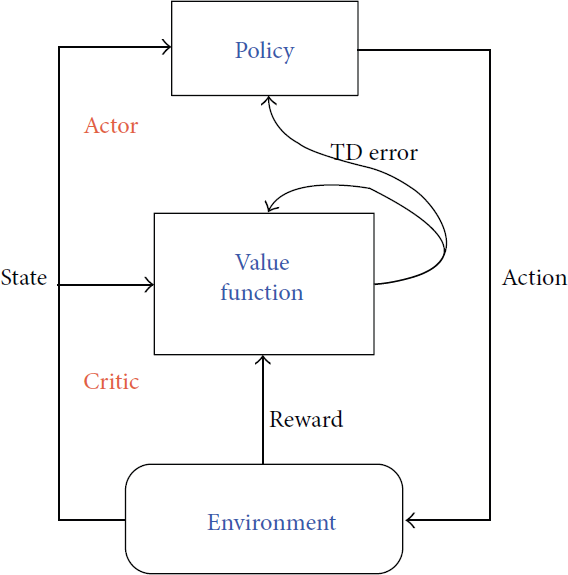
\includegraphics[width=.5\textwidth]{common_arch}
\caption{معماری رایج برای \قم}\label{fig:common_arch}
\end{figure}
در این مقاله معماریی نوین که معرفی شده است در شکل
\ref{fig:new_arch}
آمده است. همان\ طور که در این معماری نشان داده شده است یک یادگیری بروی اینکه در هر موقعیت چه کاری باید انجام شود و در سپس پرامترهای مربوط به آن عمل چگونه باید باشند و در نهایت با ترکیب خروجی\ های این دو یادگیر عمل مربوطه به محیط اعمال می\ شود.
\begin{figure}
\centering
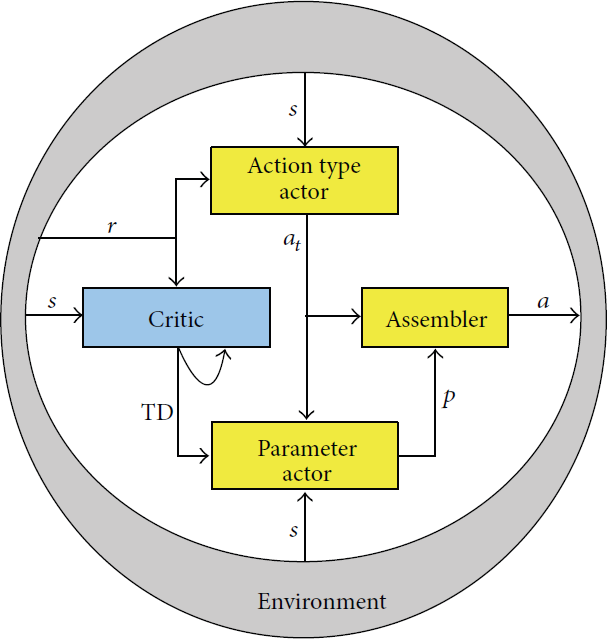
\includegraphics[width=.5\textwidth]{new_arch}
\caption{معماری معرفی شده توسط\مرجع{uc2013novel}}\label{fig:new_arch}
\end{figure}
همان\ طور که در شکل
\ref{fig:aac}
نشان داده شده است، از تخمین تابع جهت یادگیری نوع حرکت و مقادیر پارامترهای آن حرکات و منتقد استفاده شده است.\بند
در شکل
\ref{fig:aac}
به ازای یک موقعیت برای انتخاب مناسب\ ترین عمل، به تعداد اعمال که تخمین تابع داریم، عملی را انتخاب می\ کنیم که مقدار تخمین زننده\ ی آن از بقیه بیشتر باشد، بعد از انتخاب عمل به سراغ تعیین پارامترهای آن عمل می\ رویم که در آنجا نیز به تعداد پارامترهای هر عمل تخمین\ زننده داریم. این تخمین\ زننده\ ها به ازای پاداشی که از محیط می\ گیرید باید بتوانند خود را بهبود ببخشند. در آزمایش\ های این مقاله از ۳ تخمین\ زننده استفاده شده است، که عملکرد هریک از این تخمین\ زننده در شکل
\ref{fig:FA_res1}
آمده است. همان\ طور که می\ بینیم تخمین\ زننده\ ی \مق{RBF} در کل بیشتر از بقیه توانسته است که توپ را در اختیار خود داشته باشد. در شکل
\ref{fig:FA_res2}
نیز معماری معرفی شده با الگوریتم $Q(\lambda)$ مقایسه شده است، همان\ طور که از شکل سمت راست می\ بینیم با اینکه در حالت کلی الگوریتم $Q(\lambda)$ عملکرد بهتری نسبت به معماری معرفی شده داشته است ولی برای این عملکرد «اندکی» بهتر\زیرنویس{مقادیر میانگین و حداکثر مسافت اختیار توپ را در شکل سمت راست دو روش را مقایسه کنید!} باید زمانی نزدیک به ۲۴ ساعت صرف کنیم در حالی که معماری معرفی فقط در ۱۰ دقیقه توانسته سیاست خوبی را یاد بگیرد.
\begin{figure}
\centering
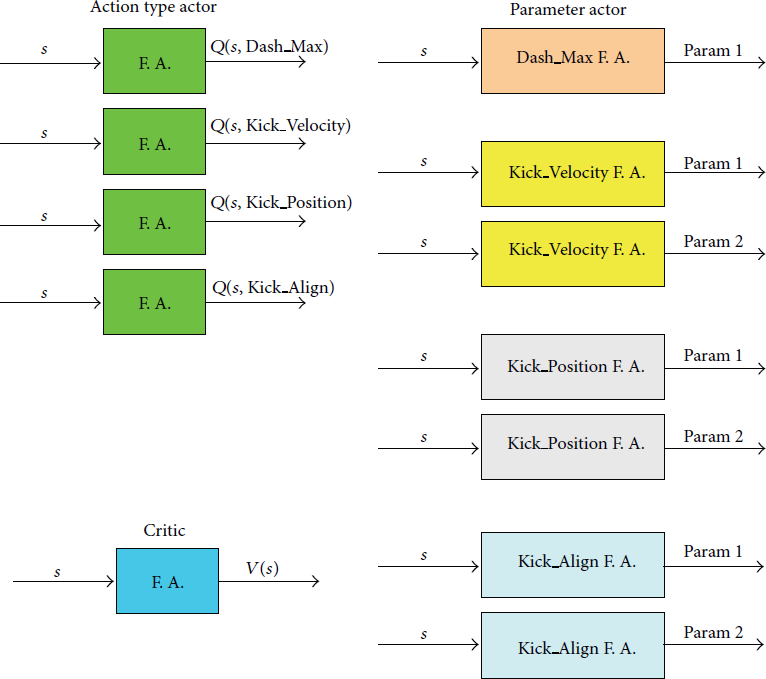
\includegraphics[width=.7\textwidth]{aac}
\caption{نحوه\ ی استفاده از تخمین تابع جهت یادگیری نوع حرکت و مقادیر پارامترهای آن حرکات و منتقد}\label{fig:aac}
\end{figure}
\begin{figure}
\centering
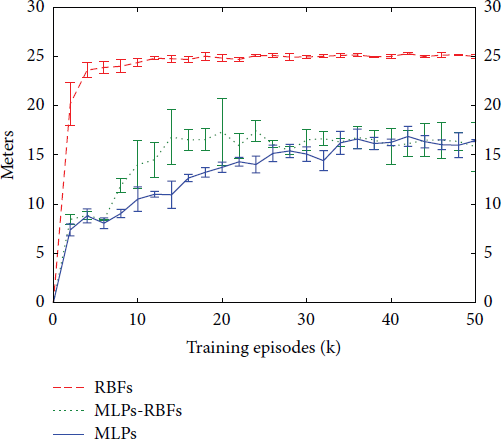
\includegraphics[width=.6\textwidth]{res1_1}
\caption{عملکرد هریک از ۳ تخمین\ زننده برحسب فاصله\ ای که ربات توانسته است که توپ را در کنترل خود داشته باشد}\label{fig:FA_res1}
\end{figure}
\begin{figure}
\centering
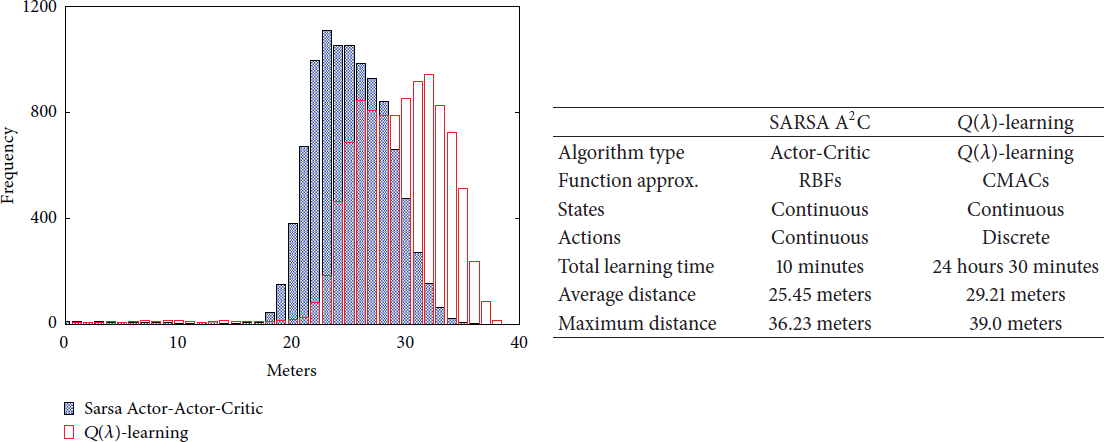
\includegraphics[width=\textwidth]{res1_2}
\caption{مقایسه\ ی معماری معرفی شده با الگوریتم \مق{$Q(\lambda)$}}\label{fig:FA_res2}
\end{figure}
\clearpage
\زیرقسمت{یادگیری قایق\ رانی}
در این کاربرد
\cite{lazaric2007reinforcement}
مفاهیم بنیادی همانند کاربرد قبلی می\ باشد، در این کاربرد نیز فرض بر این است که تعداد اعمال محدودی با مقادیر پیوسته داریم. همان\ طور که در
\ref{eq:2_A_S} تا \ref{eq:2_P_0}
آمده است، در هر موقعیت تعدادی محدود از اعمال وجود دارد که احتمال هریک از آن\ ها از توزیعی همانند $\pi$ تبعیت می\ کنند که در این توزیع احتمال انتخاب عمل $i$ام برابر با $w_i$ می\ باشد. تابع $\delta$ همان تابع دلتای دیراک می\ باشد که در صورتی که $a = a_i$ باشد مقدار ۱ و در غیر این صورت مقدار ۰ را به عنوان خروجی می\ دهد.
\begin{align}
\mathcal{A}(s) &= \{a_1,a_2,\ldots,a_N\}\label{eq:2_A_S}\\
a_i &\sim \pi^{0}(a|s)\\
\pi^{0}(a|s) &\simeq \sum_{i=1}^{N}w_i\cdot\delta(a-a_i)\label{eq:2_P_0}
\end{align}
\[a_i \in \mathcal{A}(s), w_i\in\mathcal{W}(s)\]
در ابتدا احتمال انتخاب هر عمل در از توزیع یکنواخت پیروی می\ کند و به مرور احتمال انتخاب\ ها متناسب به بازخوردی که از محیط می\ گیرد ممکن است تغییر کنند. الگوریتم ارائه شده همانند الگوریتم\ های معمول \قم می\ باشد فقط با این تفاوت که هنگام انتخاب عمل در هر موقعیت، عملی را انتخاب می\ کند که دارای بیشترین وزن($w_i$) باشد و برای بروزرسانی وزن\ ها از رابطه\ ی
\ref{eq:update_w}
استفاده می\ کنیم. الگوریتم ارائه شده در شکل
\ref{fig:alg2}
آمده است.\بند
\begin{align}
w_i^{t+1} &= w_i^t {e^{\Delta Q^{t+1}(s, a_i) \over \tau} \over \sum_{j = 1}^Nw_je^{\Delta Q^{t+1}(s, a_j) \over \tau}}\label{eq:update_w}\\
\Delta Q^{t+1}(s, a_i) &= Q^{t+1}(s, a_i) - Q^{t}(s, a_i)\nonumber
\end{align}
\begin{figure}
\centering
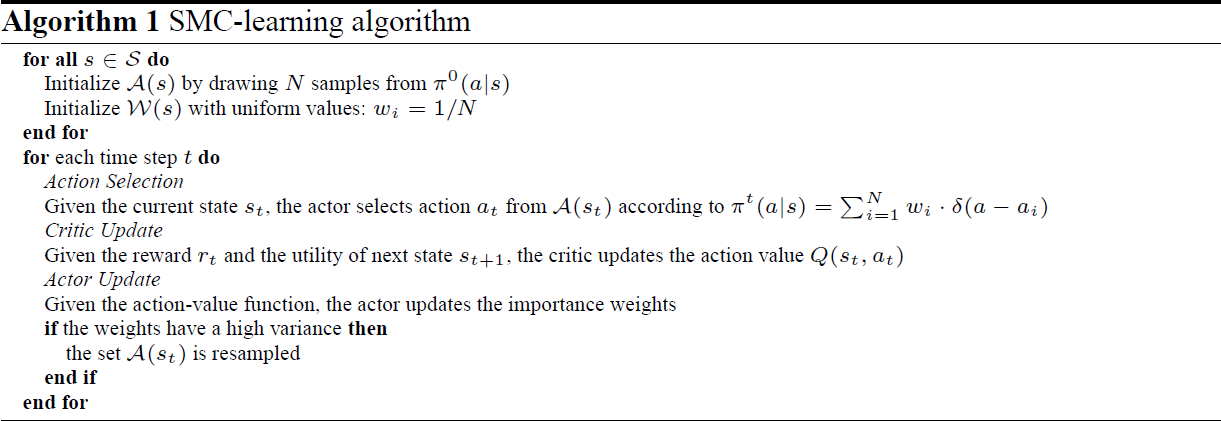
\includegraphics[width=\textwidth]{alg2}
\caption{الگوریتم ارائه شده برای کاربرد یادگیری قایق\ رانی}\label{fig:alg2}
\end{figure}
مساله\ ای که در این مقاله مطرح شده است، مساله\ ی یادگیری قایق\ رانی است، همان\ طور که در شکل
\ref{fig:boat_prob}
می\ بینیم، قایق توسط زاویه\ ی فرمان و اختلاف نوک قایق با افق هدف مشخص می\ شود، همچنین به عنوان اغتشاش یک جریان آبی نیز در رودخانه در جریان است، هدف این است که قایق در ناحیه\ ی مشخص شده بتواند لنگر بیاندازد.
\begin{figure}
\centering
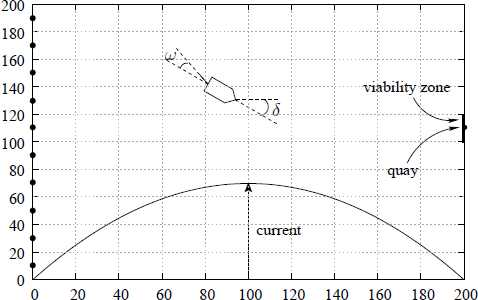
\includegraphics[width=.5\textwidth]{boat_prob}
\caption{تعریف مساله\ ی کاربرد یادگیری قایق\ رانی}\label{fig:boat_prob}
\end{figure}
همان\ طور که در شکل
\ref{fig:res2}
می\ بینیم، الگوریتم ارائه شده توانسته زودتر از الگوریتم \مق{SARSA} همگرا شود و نسبت به الگوریتم \مق{Q} پاداش\ های بیشتری توانسته کسب کند.
\begin{figure}
\centering
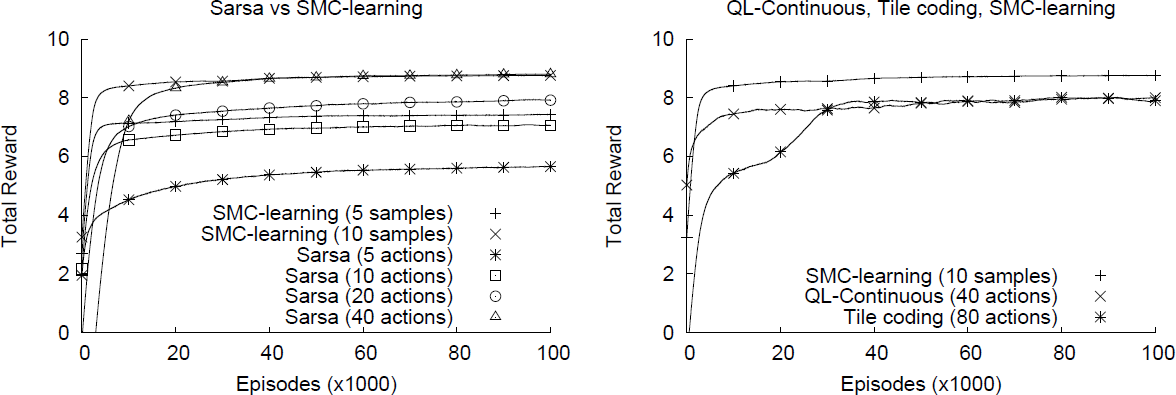
\includegraphics[width=\textwidth]{res2}
\caption{مقایسه\ ی الگوریتم ارائه شده(شکل \ref{fig:alg2}) با الگوریتم\ های \مق{SARSA} و \مق{Q}}\label{fig:res2}
\end{figure}
\قسمت{نتیجه\ گیری}
در این گزارش به بررسی دلایلی که چرا الگوریتم\ های معمول \قم نمی\ توانند برای کاربردهای دنیای واقعی استفاده شوند، پرداختیم؛ سپس به معرفی دو کاربرد متفاوت از کاربردهای دنیای واقعی پرداختیم و همان\ طور که دیدیم بسته به نوع مساله باید تغییرات/روش\ هایی ارایه داد که متناسب با مساله باشد و با مقادیر پیوسته\ ی موقعیت و اعمال بتواند اجرای خوبی داشته باشد -- روش\ های معمول توانایی کار با مسایل با مقادیر پیوسته را ندارند.
\قسمت{مراجع}
\nocite{*}
\renderref{reference}
\end{document}
